\documentclass{beamer} % beamer is the document class for presentation slides

% languages typesetting rules
\usepackage{polyglossia} % handle multiple languages typesetting rules
\setdefaultlanguage{french} % this presentation is in french
\setotherlanguages{english,greek} % this presentation sometimes uses english and greek texts
\newfontfamily\greekfont[Script=Greek]{Linux Libertine O} % we need a special font for greek text
\newfontfamily\greekfontsf[Script=Greek]{Linux Libertine O} % same, but sans serif

\usepackage{hyperref} % commands such as \href, \url, etc.
\usepackage[backref=true]{biblatex} % bibliography handling
\usepackage{csquotes} % biblatex extensions for non-english languages
\usepackage{tipa} % International Phonetic Alphabet symbols and helpers
\usepackage{caption} % more control over captions
\usepackage{ccicons} % icons for Creative-Commons licenses

\usetheme{Warsaw}
\useoutertheme{infolines} % Display the slides number in the footline (and a smaller header)

% Add a tableofcontent slide before each subsection, highlighting the section we're at
\AtBeginSection[]{
    \frame{\tableofcontents[currentsection]}
}

% define the \ipa command that switches to english typography rules before
% calling \textipa (which gets confused by french typography rules)
\newcommand{\ipa}[1] {
    \selectlanguage{english}
    \textipa{#1}
}

% Bibliography configuration
\bibliography{references}

\title{Écriture de documents avec \LaTeX{}}
\subtitle{\texorpdfstring{\small{\emph{D'après une conférence de Didier Verna}\cite{latexDV}}}
                         {D'après une conférence de Didier Verna}}
\titlegraphic{\large{\href{https://creativecommons.org/licenses/by-sa/4.0/}{\ccbysa}}}
\institute{EPITA}
\author{
    % The authors information appear in the first page of the document but also
    % in the pdf's metadata. A lot of stuff isn't allowed in the metadata
    % (links, line breaks, etc.) so we must define two alternatives, one for the
    % document page and one for the metadata, this is done with the
    % \texordpdfstring command
    \texorpdfstring
    { % Nicely formatted author information
        Paul Hervot\\
        \href{mailto:paul.hervot@epita.fr}{\nolinkurl{paul.hervot@epita.fr}}
    }{ % A simpler version for the pdf's metadata
        Paul Hervot
    }
}
\date{3 septembre 2019}

\begin{document}
\frame{\titlepage{}}

\section{Introduction}
\subsection{\TeX}
\begin{frame}{\TeX}
    \begin{description}
        \item[Nom :] symbolise les lettres \textgreek{τεχ}, abbréviation de \textgreek{τέχνη}
        \item[Objectif :] mise en forme typographique entièrement informatique
        \item[Création :] Donald Knuth, 1977-1989
        \item[Prononciation :] \ipa{[tEx]}
    \end{description}

    \begin{figure}[position]
        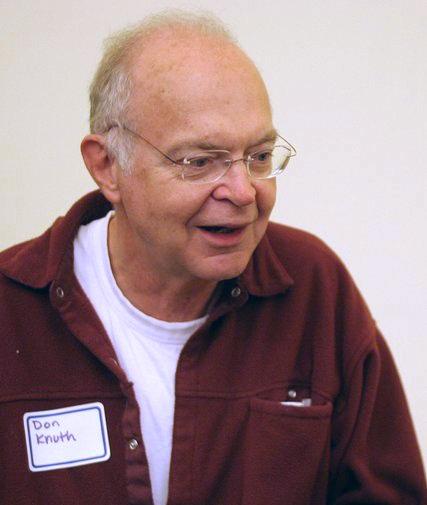
\includegraphics[height=0.5\textheight]{img/knuth}
        \caption*{Donald Knuth, en 2005\cite{knuthpic}}
    \end{figure}
\end{frame}

\subsection{\LaTeX}
\begin{frame}{\LaTeX}
    \begin{description}
        \item[Nom :] abbréviation de Lamport-\TeX
        \item[Objectif :] ensemble de macros (raccourcis) pour \TeX
        \item[Création :] Leslie Lamport, 1983
        \item[Prononciation :] \ipa{["lA:tEx]} ou \ipa{["leI:tEx]}
    \end{description}

    \begin{figure}[position]
        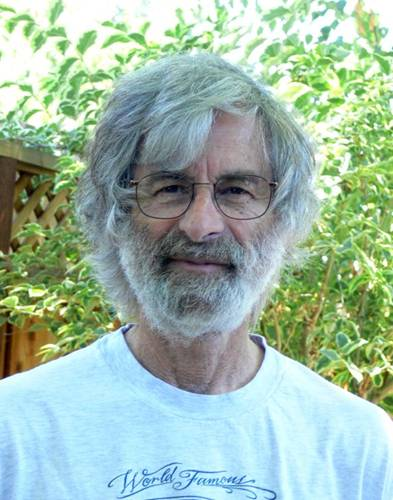
\includegraphics[height=0.5\textheight]{img/lamport}
        \caption*{Leslie Lamport, vers 2014}
    \end{figure}
\end{frame}

\section{Conclusion}
\subsection{Références}
\begin{frame}[allowframebreaks]{Bibliographie}
    \printbibliography{}
\end{frame}
\end{document}
